% !TeX root = ../main.tex

\chapter{Compressed-Domain Visual Odometry}\label{chapter:method}

\section{System Overview}

The examined pipeline separates image-dependent preparation from compressed-domain
estimation, as summarized in \autoref{fig:system-pipeline}. Offline preparation
encodes native images into temporal H.264 streams and rectified images into
stereo streams. The extraction software decodes these streams to obtain their
motion-vector metadata. Only codec side information, calibration, masks, and
timing metadata enter the tracking frontend and pose estimator.
Temporal vectors propose motion, shifted stereo encodings provide metric
depth, and robust registration validates the resulting 3D-3D associations.
Confirmed identities are converted into observations for a windowed
visual-odometry backend.

\begin{figure}[htbp]
  \centering
  \resizebox{\textwidth}{!}{%
  \begin{tikzpicture}[
      prep/.style={draw=TUMBlue, rounded corners, align=center, fill=white,
        minimum height=9mm, text width=25mm, font=\small},
      estimation/.style={draw=TUMBlue, rounded corners, align=center, fill=white,
        minimum height=10mm, text width=22mm, font=\small},
      flow/.style={->, thick, color=TUMDarkGray}]
    \node[anchor=west,font=\small\bfseries,color=TUMSecondaryBlue]
      at (-0.35,4.55) {Offline preprocessing: image intensities available};
    \draw[dashed,rounded corners,color=TUMSecondaryBlue]
      (-0.50,0.45) rectangle (13.05,4.35);

    \node[prep] (images) at (1.00,2.35) {Native stereo images\\and calibration};
    \node[prep] (temporal) at (4.35,3.35) {Temporal H.264\\forward and reverse};
    \node[prep] (rectify) at (4.35,1.35) {Rectification\\+ masks};
    \node[prep] (stereoencode) at (7.75,1.35) {Shifted stereo H.264\\I-P-P streams};
    \node[prep] (products) at (11.45,2.35) {Encoded streams,\\masks +\\calibration};
    \draw[flow] (images.east) -- ++(0.35,0) |- (temporal.west);
    \draw[flow] (images.east) -- ++(0.35,0) |- (rectify.west);
    \draw[flow] (rectify) -- (stereoencode);
    \draw[flow] (temporal.east) to[out=0,in=90] (products.north);
    \draw[flow] (stereoencode.east) to[out=0,in=-90] (products.south);

    \node[anchor=west,font=\small\bfseries,color=TUMSecondaryBlue]
      at (-0.35,0.05) {Frontend and pose estimation: no image intensities};
    \draw[dashed,rounded corners,color=TUMSecondaryBlue]
      (-0.50,-3.00) rectangle (10.10,-0.15);
    \node[prep] (extract) at (11.65,-1.60) {Decode frames +\\extract MV metadata\\(uses pixels)};
    \node[estimation] (filter) at (8.80,-1.60) {Median + reciprocal\\filtering};
    \node[estimation] (stereolookup) at (6.15,-1.60) {Stereo depth\\at both\\endpoints};
    \node[estimation] (registration) at (3.50,-1.60) {TEASER++ +\\track identity};
    \node[estimation] (backend) at (0.85,-1.60) {Suppression +\\rigid-flow BA};
    \draw[flow] (products.south) -- (extract.north);
    \draw[flow] (extract) -- (filter);
    \draw[flow] (filter) -- (stereolookup);
    \draw[flow] (stereolookup) -- (registration);
    \draw[flow] (registration) -- (backend);
  \end{tikzpicture}}
  \caption[Processing pipeline and pixel-access boundary]{Processing pipeline and pixel-access boundary. Rectification and
  both H.264 paths operate on images before evaluation. Native images feed the
  forward/reverse temporal encodings, while rectified images feed the shifted
  stereo encodings. The extractor reconstructs image pixels, which are not
  passed to the frontend. The pixel-free boundary encloses correspondence
  filtering, stereo lookup, association, and pose estimation; these stages
  consume only side information, masks, timing data, and calibrated geometry.}
  \label{fig:system-pipeline}
\end{figure}

\section{Input and Pixel-Access Boundary}

For each timestamp, the estimator receives temporal motion vectors from the
forward and reverse encodings, stereo motion vectors from the shifted I-P-P
encodings, the width and height of every prediction block, reference direction,
fractional displacement and frame type. It additionally receives the two-camera
calibration, synchronized timestamps, the virtual rectification model, and the
two rectification validity masks. These quantities are sufficient to express
codec supports in native camera coordinates and to form calibrated rays.

In compressed-domain operation, image loading is disabled before observations
enter the frontend. The frontend neither constructs image pyramids nor
runs FAST, KLT, patch alignment, descriptor extraction, or a photometric test.
Image intensities are used to generate the H.264 streams during offline
preprocessing, and the extraction software reconstructs images while reading
codec side information. Neither the tracking frontend nor pose estimation consumes
those intensities. The Shi-Tomasi and blur measurements reported later
are likewise post-hoc diagnostics and are not available to pose estimation.

\section{Stereo Rectification and Video Preprocessing}

Rectification is constructed separately for each supplied stereo calibration.
The camera supplying temporal track candidates is designated the anchor camera
$A$, and the other view is the stereo camera $S$. Let
${}^{A}\mathbf{t}_{S}$ be the position of the stereo camera expressed in the
anchor-camera frame.
The horizontal axis of the virtual camera is
$\mathbf{e}_x={}^{A}\mathbf{t}_{S}/\lVert{}^{A}\mathbf{t}_{S}\rVert$.
The sum of the two native optical axes, expressed in the anchor-camera frame,
is projected onto
the plane orthogonal to $\mathbf{e}_x$ and normalized to form
$\mathbf{e}_z$; $\mathbf{e}_y=\mathbf{e}_z\times\mathbf{e}_x$ completes the
orientation. This produces a common view direction while making the calibrated
baseline horizontal.

Both cameras are remapped into the same undistorted pinhole projection. Its
resolution equals the native EuRoC resolution, its principal point is the image
centre, and its common focal length is the smallest of the four native horizontal
and vertical focal parameters. Each virtual ray is rotated into the respective
native camera and projected with that camera's calibrated distortion model.
Bilinear sampling produces the offline rectified images. Pixels for which this
mapping is invalid are set to zero, and a binary validity mask for each camera is
stored with the virtual intrinsics and rotations. During estimation, an entire
codec block is rejected if either of its rectified supports intersects an invalid
region.

Camera streams are paired by their recorded nanosecond timestamps. If one camera
contains an unmatched terminal image, only that unpaired timestamp is removed
from the longer metadata stream; both the temporal video and its reverse
counterpart are generated from the resulting ordered timestamp list. EuRoC has
two cameras, so its calibrated pair is used directly. For a dataset with more
than two cameras, one calibrated pair would have to be designated as the anchor
and stereo views; additional cameras would remain outside the
Passthrough+-derived depth stage.

\section{Codec-Domain Stereo Correspondences}

Only the sparse encoder-stereo stage of Passthrough+~\cite{chaurasia2020passthrough} is adapted. The shifted views are represented as independent full-frame encodings rather than subframes of one hardware-encoder mosaic. Temporal motion-search and partition settings are retained, while the reference structure, rate control, and encoded frame rate follow the stereo configuration in \autoref{chapter:experimental-methodology}. Each EuRoC camera pair is remapped into a calibration-specific common virtual projection before encoding. During estimation, stereo motion vectors are queried only at temporal candidate locations; their endpoints are converted back to native camera rays and triangulated with the calibrated baseline.

The original hemispherical depth grid, Laplacian densification, stereoscopic rendering, and pixel-based subpixel refinement are not used. Nor is its temporal depth-map propagation: Passthrough+ projects the previous depth map using a headset pose obtained from an independent SLAM system~\cite{chaurasia2020passthrough}, whereas no external pose estimate is available here. Sparse stereo depths instead serve as geometric support for temporal association and visual odometry.

Writing $L$ for the anchor view and $R$ for the stereo view, three horizontal
pre-shifts, 0, 8, and 32 pixels, are combined with four codec
grid phases, $(0,0)$, $(4,0)$, $(0,4)$, and $(4,4)$ pixels. The resulting twelve
independent streams contain repeated triples
\begin{equation}
  I(L_t^{s,g}),\quad P(R_t^g),\quad P(L_t^{s,g}),
\end{equation}
where $s$ denotes the disparity pre-shift and $g$ the grid phase. With one
reference frame, the first P-frame supplies left-to-right predictions and the
second supplies right-to-left predictions. The known artificial shifts are
removed from the reported block coordinates. Left-to-right and right-to-left
blocks are paired one-to-one when their supports overlap and their componentwise
cycle error is at most 1.0 pixel. The intersection of the two supports becomes
the validated rectangle.

A native anchor-camera query $\mathbf{u}$ is first unprojected, rotated into the virtual
frame, and projected onto the rectified grid. Every variable-sized codec block
whose source rectangle contains this location is considered; blocks are not
expanded into per-pixel points. Applying that block's fractional motion vector
gives a candidate in the rectified right view. Both endpoints must lie in valid
rectification support, and their vertical displacement in the common grid must
not exceed one pixel. The encoded right endpoint is then converted to a native
stereo-camera ray. The frontend triangulates distances along unit native-camera
bearings. Candidates are rejected when their calibrated epipolar error exceeds
$0.005$, triangulation is degenerate, either depth is at most
$\SI{0.333}{\metre}$, the anchor-camera depth exceeds $\SI{30}{\metre}$, or reprojection
into the stereo camera differs from the candidate by more than $1.5$ pixels.

When several encodings or overlapping variable-size blocks cover the query, one
stereo observation is returned. Its ranking cost is
\begin{equation}
  C = e_{\mathrm{repr}} + e_{\mathrm{epi}}
      + 10^{-4}wh + 10^{-3}d_c,
\end{equation}
Here $e_{\mathrm{repr}}$ is the stereo reprojection distance in pixels, and
$e_{\mathrm{epi}}=|\hat{\mathbf b}_L^{\mathsf T}\mathbf E\hat{\mathbf b}_R|$
is a dimensionless epipolar residual. The bearings are unit vectors in their
native camera frames, and $\mathbf E$ is the essential matrix formed from the
calibrated relative rotation and unit baseline direction.
The product $w h$ is block area and $d_c$ is the squared, block-size-normalized
distance from the query to the block centre. This preference resolves duplicate
codec hypotheses locally; the later suppression stage handles geometrically
indistinguishable temporal measurements.

\subsection{Grid Sampling and Disparity Pre-Shifts}

The grid phases and horizontal pre-shifts address two different aspects of
stereo correspondence. Grid phases increase spatial sampling density.
Applying the same phase $g$ to both views moves the codec's sampling grid
relative to the scene while preserving disparity. In the eight-pixel sampling
example used by Passthrough+~\cite{chaurasia2020passthrough}, the phases
$(0,0)$, $(4,0)$, $(0,4)$, and $(4,4)$ interleave into a grid with four-pixel
spacing in both directions, as shown in \autoref{fig:stereo-grid-interleaving}.
The combined samples refine spatial coverage. This spacing describes the
sampling construction; the encoded prediction blocks and their validated
intersections retain variable sizes.

\begin{figure}[htbp]
  \centering
  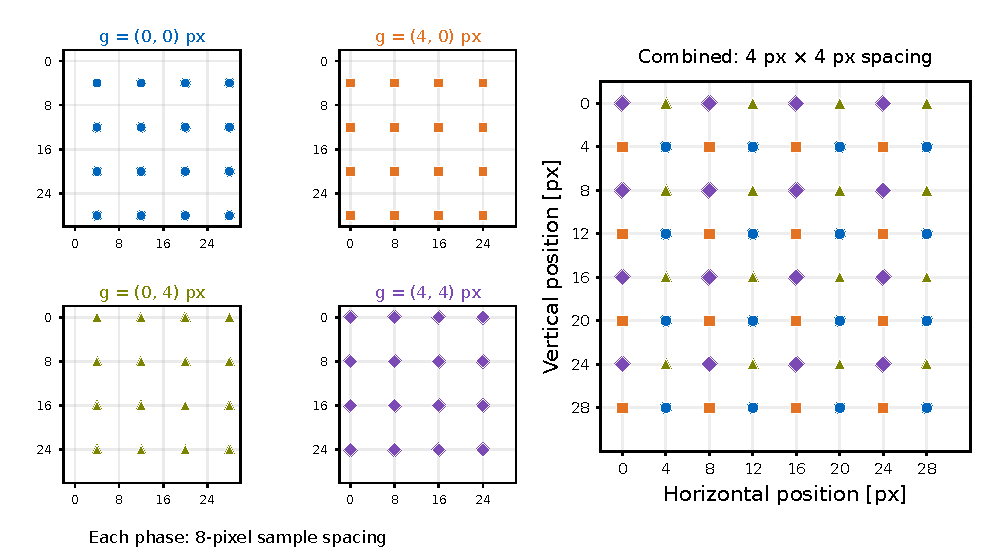
\includegraphics[width=\textwidth]{figures/method/stereo-grid-phase-interleaving.pdf}
  \caption[Finer spatial sampling through grid-phase interleaving]{Grid-phase interleaving, illustrated for an eight-pixel base grid.
  The four phases sample different positions in the same image coordinates.
  Their union has four-pixel spacing horizontally and vertically. Colour and
  marker shape identify the originating phase. The same phase is applied to
  both stereo views, so it changes sampling position without changing disparity.}
  \label{fig:stereo-grid-interleaving}
\end{figure}

Horizontal pre-shifts change the displacement presented to the encoder.
Passthrough+ reports that encoders favour short motion vectors, making
large disparities from nearby surfaces harder to recover~\cite{chaurasia2020passthrough}.
For disparity $d=u_L-u_R$, shifting the left image by $s$ pixels presents
$d-s$ to the encoder. The known shift is restored before triangulation.
With focal length $f_x$ and baseline $B$, rectified axial depth satisfies
\begin{equation}
  Z = \frac{f_x B}{d}, \qquad
  |d-s| = \left|\frac{f_x B}{Z}-s\right|.
  \label{eq:stereo-shift-depth}
\end{equation}
Here $Z$ is axial depth in the virtual rectified camera, used to interpret the
pre-shift examples and depth visualizations. The tracking frontend instead
triangulates distance along native-camera unit bearings, denoted $\lambda$
below.

\autoref{fig:stereo-shift-success-failure} shows two locations whose depth is
recovered by different pre-shifts. At the EMH01 location at \SI{135}{\second},
a disparity of 29.25 pixels gives $Z\approx\SI{1.31}{\metre}$. The 32-pixel
pre-shift reduces the required displacement to 2.75 pixels and provides an
accepted match. The displayed 0- and 8-pixel proposals instead have a vertical
error of 1.75 pixels and fail the one-pixel check. At the EMH02 location at
\SI{95}{\second}, disparity is 8.50 pixels and $Z\approx\SI{4.52}{\metre}$;
the 8-pixel pre-shift reduces the required displacement to 0.50 pixels and
supplies the depth.

For each location, all four grid phases are checked: neither of the other
pre-shifts returns an accepted block covering that query. Thus, a pre-shift
can determine whether a particular scene location supplies depth, and the
useful pre-shift changes with disparity. Local appearance and codec decisions
also affect availability, so useful depth ranges can overlap.
The illustrated matches pass rectification-mask, vertical-displacement,
reciprocal-cycle, and one-to-one overlap checks; they precede temporal tracking
and backend landmark selection. An overview of the correspondences from all
twelve transforms on a later EMH02 frame is given in
\autoref{fig:stereo-all-shifts}.

\begin{figure}[p]
  \centering
  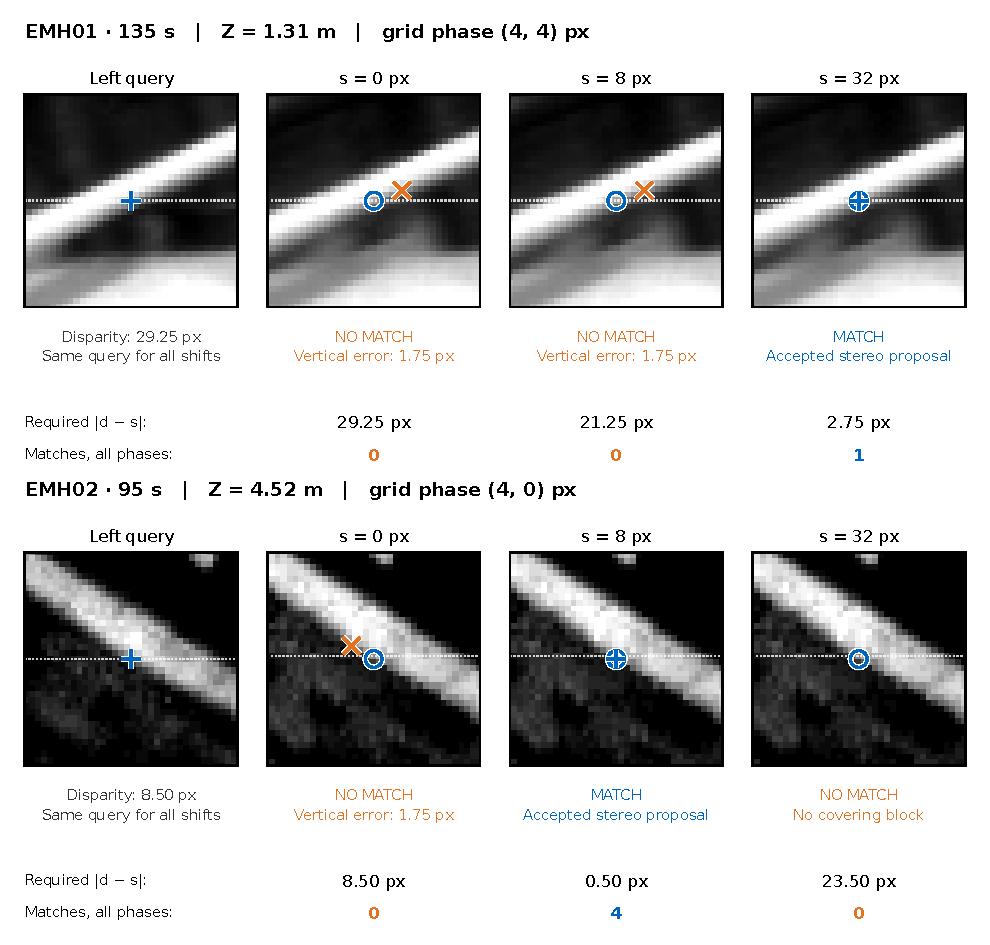
\includegraphics[width=\textwidth]{figures/method/stereo-shift-exclusive-depths.pdf}
  \caption[Depth recovery at different pixel pre-shifts]{Pre-shift-dependent depth recovery at two later scene locations.
  Each row holds the left query and displayed grid phase fixed. Blue circles
  repeat the right-image match supplied by the successful pre-shift; orange
  crosses mark rejected proposals. The dotted line is the query's epipolar
  row. The required residual $|d-s|$ is computed from the recovered disparity;
  the counts below include all four grid phases. Left and right crops within
  a row share one grayscale display scale.}
  \label{fig:stereo-shift-success-failure}
\end{figure}

\autoref{fig:stereo-depth-examples} and
\autoref{fig:stereo-depth-late-machine-hall} show depth renderings in three
scenes: EV101 at \SI{60}{\second}, EMH01 at \SI{115}{\second}, and EMH02 at
\SI{135}{\second}. A separate grayscale depth inset is placed inside each
rectified scene image. Stereo-block support surviving the rectification and
bidirectional checks is sampled on a four-pixel grid. Each supported sample
displays calibrated axial depth, using the median where several blocks cover
the same location. Brighter values indicate nearer surfaces; black marks
locations without a displayed sample. Unsupported regions are left unfilled.
These post-hoc renderings make the codec-derived geometry inspectable;
grayscale intensity is not passed to the estimator.

\begin{figure}[htbp]
  \centering
  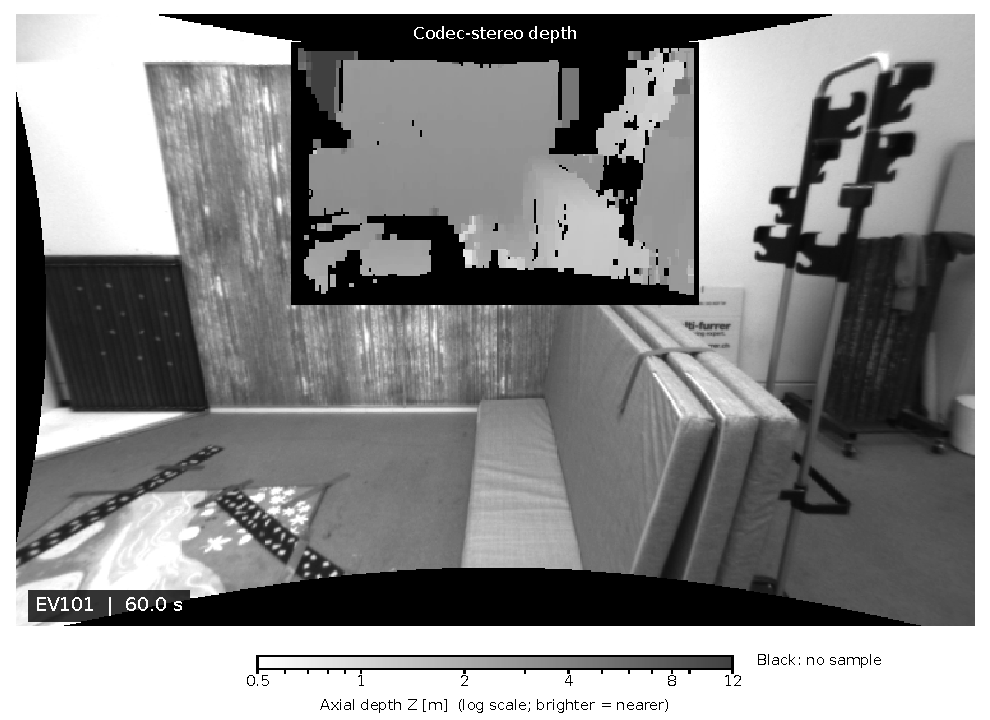
\includegraphics[width=\textwidth]{figures/method/depth-inset-ev101-f1200.pdf}
  \caption[Codec-stereo depth map on EV101]{Codec-stereo depth for EV101 at \SI{60}{\second}. The inset shows
  the full field of view on a four-pixel sampling grid, with nearer surfaces
  brighter on the logarithmic depth scale. Black marks unsupported samples;
  depths outside the displayed \SIrange{0.5}{12}{\metre} range are clipped
  only for grayscale visualization.}
  \label{fig:stereo-depth-examples}
\end{figure}

\begin{figure}[p]
  \centering
  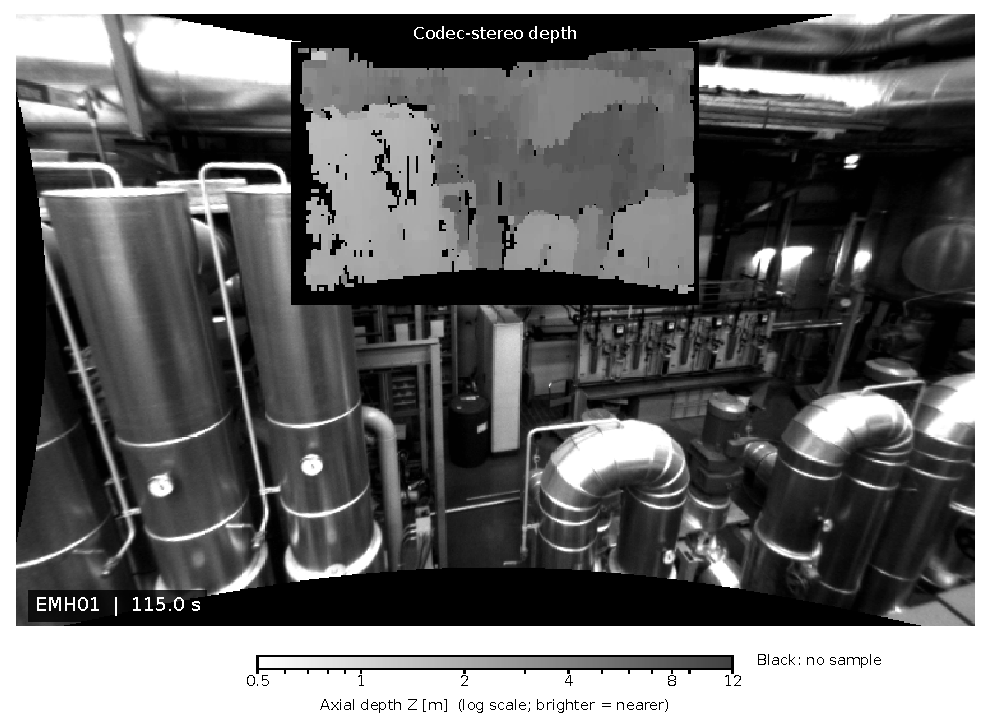
\includegraphics[width=0.80\textwidth]{figures/method/depth-inset-emh01-f2300.pdf}
  \par\medskip
  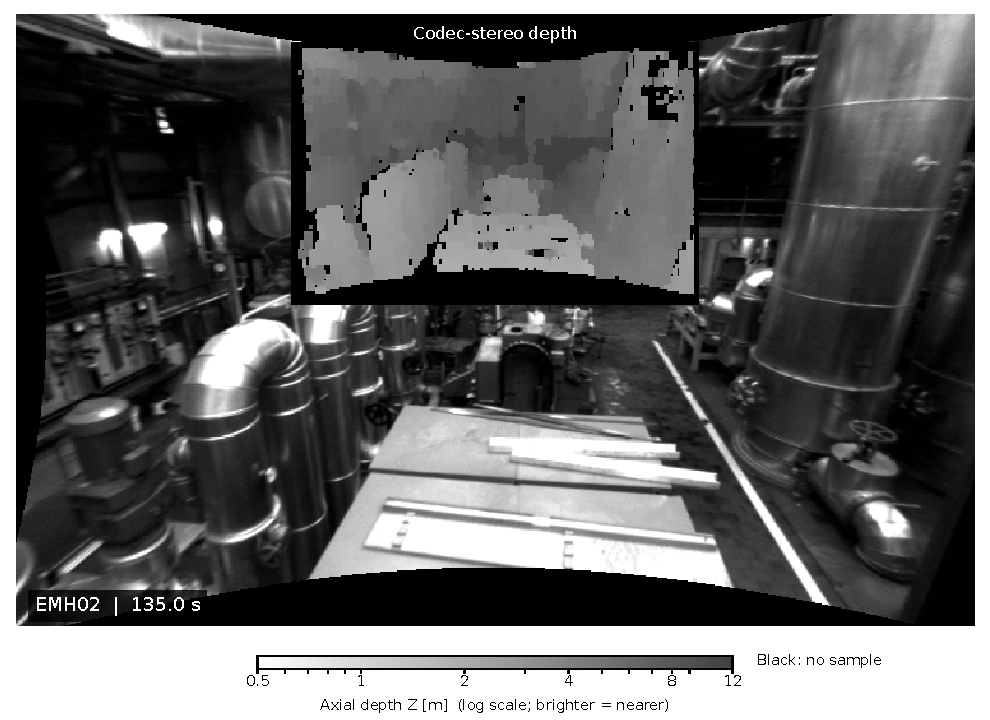
\includegraphics[width=0.80\textwidth]{figures/method/depth-inset-emh02-f2700.pdf}
  \caption[Codec-stereo depth maps in later Machine Hall scenes]{Additional codec-stereo depth maps in later Machine Hall scenes:
  EMH01 at \SI{115}{\second} (top) and EMH02 at \SI{135}{\second} (bottom).
  Both use the grayscale scale and sampling convention of
  \autoref{fig:stereo-depth-examples}. The separate depth insets distinguish
  nearby equipment from more distant structure while retaining unsupported
  regions in black.}
  \label{fig:stereo-depth-late-machine-hall}
\end{figure}

\section{Temporal Motion-Vector Candidates}

Motion vectors are read from the H.264 side data with their reference direction,
block dimensions, integer numerator, and scale. Only vectors referencing the
preceding encoded frame are used. Dividing the numerator by the scale preserves
the fractional current-to-reference displacement $\mathbf v$. In the forward
encoding, a coding-block centre $\mathbf q_t$ corresponds to the reference-support
centre $\mathbf q_{t-1}=\mathbf q_t+\mathbf v$. The temporal candidate runs from
$\mathbf q_{t-1}$ to $\mathbf q_t$, with forward displacement
$\mathbf m=-\mathbf v$. Later continuation may apply a covering block's
displacement to an established track location; it does not repeatedly snap that
location back to the block centre.

The compression-artifact filter tests local agreement without consulting the
image. Motion vectors are accumulated into a $16\times16$-pixel grid and their
two displacement components are averaged independently in each occupied cell.
For a cell $q$, let $\bar{\mathbf v}_q$ denote this mean and let
$\widetilde{\mathbf v}_q$ be the componentwise median of the occupied cells in
its $3\times3$ neighbourhood. Provided that at least three neighbouring cells
are occupied, every vector assigned to $q$ receives the score
\begin{equation}
  d_{\mathrm{med}}(q)
  = \left\lVert\bar{\mathbf v}_q-\widetilde{\mathbf v}_q\right\rVert_2.
\end{equation}
It is retained when $d_{\mathrm{med}}\leq5$ pixels. Border cells, cells without
sufficient neighbourhood support, out-of-image endpoints, and endpoints in
masked-out image regions are rejected. The result is illustrated in
\autoref{fig:median-filter-example}: the large magenta vectors disagree with
the coherent downward motion that dominates their neighbourhoods.

\begin{figure}[htbp]
  \centering
  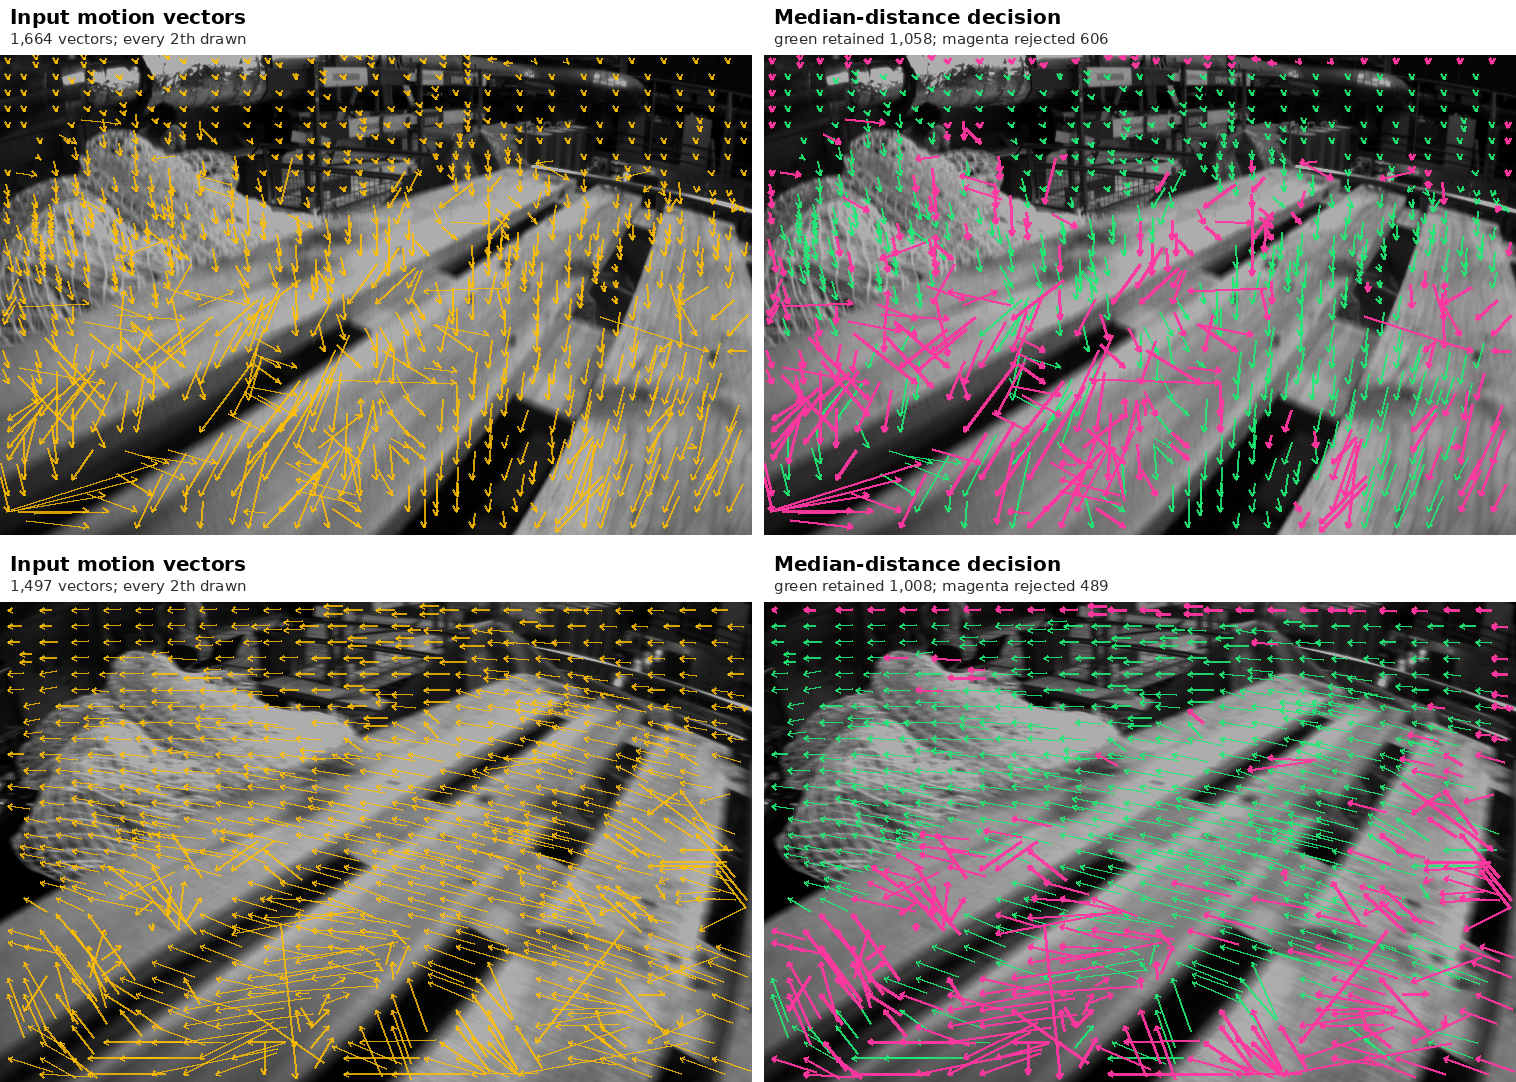
\includegraphics[width=\textwidth]{figures/method/median-filter-example}
  \caption[Median filtering of temporal motion vectors]{Examples of median-filter decisions on two EMH01 frames. In each row the
  left panel shows the input field; on the right, retained vectors are green and
  rejected vectors are magenta. Arrows use the measured displacements; dense
  populations are deterministically subsampled only for legibility.}
  \label{fig:median-filter-example}
\end{figure}

The forward encoding supplies $t-1\rightarrow t$ motion. A second video encoded
in reverse image order supplies the same interval from the opposite temporal
direction; its vectors and timestamps are inverted back into forward-time
coordinates. The fixed single-reference encoder setting prevents a temporal
vector from silently spanning more than one frame. At an I-frame boundary, the
available direction is used if exactly one encoding supplies inter prediction.
If neither direction supplies a candidate, the affected tracks terminate rather
than receiving a copied or pixel-derived displacement.

A motion vector describes a block prediction, not the identity of a scene point
inside that block. Naively assigning a persistent ID to whichever block covers
the previous sample can therefore fail in two distinct ways. First,
the selected block can continue to produce plausible motion after its displacement
has ceased to follow the same localized structure. \autoref{fig:mv-feature-departure-example}
shows this effect over fourteen transitions on a strong-gradient railing edge.
The codec path and a post-hoc KLT track initially agree, then separate
progressively while raw codec vectors remain available.

\begin{figure}[htbp]
  \centering
  \begin{minipage}[t]{0.485\textwidth}\centering
    \textbf{Track initialization}\\[-0.15em]
    {\small stereo depth: $1.98$ m}\par\smallskip
    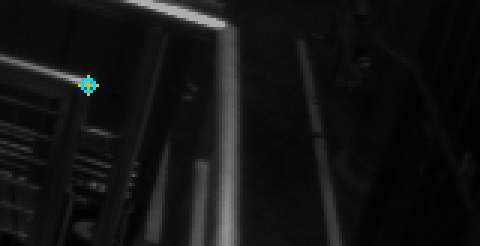
\includegraphics[width=\linewidth]{figures/method/mv-divergence-1}
  \end{minipage}\hfill
  \begin{minipage}[t]{0.485\textwidth}\centering
    \textbf{Four transitions later}\\[-0.15em]
    {\small MV to KLT gap: $0.86$ px}\par\smallskip
    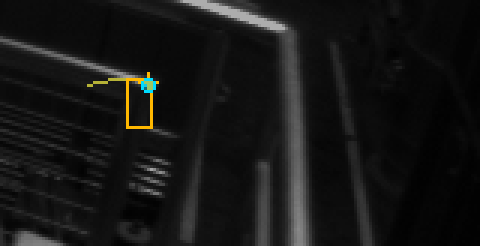
\includegraphics[width=\linewidth]{figures/method/mv-divergence-2}
  \end{minipage}

  \medskip
  \begin{minipage}[t]{0.485\textwidth}\centering
    \textbf{Nine transitions later}\\[-0.15em]
    {\small MV to KLT gap: $6.68$ px}\par\smallskip
    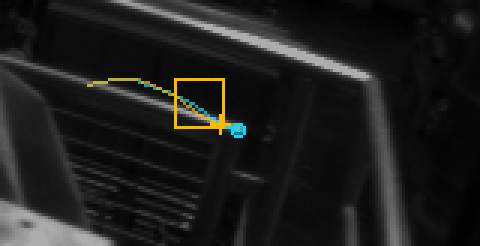
\includegraphics[width=\linewidth]{figures/method/mv-divergence-3}
  \end{minipage}\hfill
  \begin{minipage}[t]{0.485\textwidth}\centering
    \textbf{Fourteen transitions later}\\[-0.15em]
    {\small MV to KLT gap: $16.28$ px}\par\smallskip
    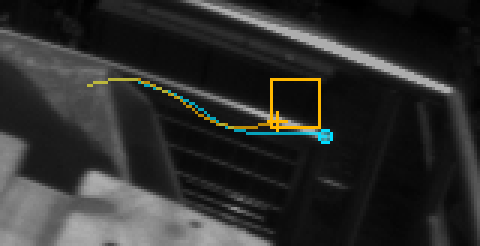
\includegraphics[width=\linewidth]{figures/method/mv-divergence-4}
  \end{minipage}
  \caption[Drift of a propagated codec sample from an image feature]{Failure of naive ID propagation on EMH01. Both diagnostic tracks
  start at the same selected image feature. Orange repeatedly applies the raw,
  unfiltered H.264 vector whose source block covers the preceding point; its
  rectangle shows that step's destination block support. Cyan is an OpenCV
  pyramidal KLT track computed
  after the experiment and retained only while its per-step forward-backward
  error is at most one pixel. It is diagnostic and is not consumed by the
  estimator. The nearest accepted compressed-stereo sample is $3.43$ pixels
  from the birth location and estimates a depth of $1.98$ metres. The trails
  show the full histories up to each displayed stage.}
  \label{fig:mv-feature-departure-example}
\end{figure}

Second, local inter-prediction support can disappear although the tracked image
structure remains visible. In \autoref{fig:mv-abrupt-stop-example}, raw motion
vectors remain present in the destination image at the first unsupported
transition, but none has a source block covering the previously propagated
point. The KLT diagnostic remains stable over the subsequent observations. The
trace alone does not identify whether this local absence
was caused by an intra-coded block, a partition change, or another encoder
decision. It nevertheless demonstrates why an absent vector cannot be equated
with an absent scene point.

\begin{figure}[htbp]
  \centering
  \begin{minipage}[t]{0.485\textwidth}\centering
    \textbf{Complete paths}\\[-0.15em]
    {\small codec path terminates; KLT continues}\par\smallskip
    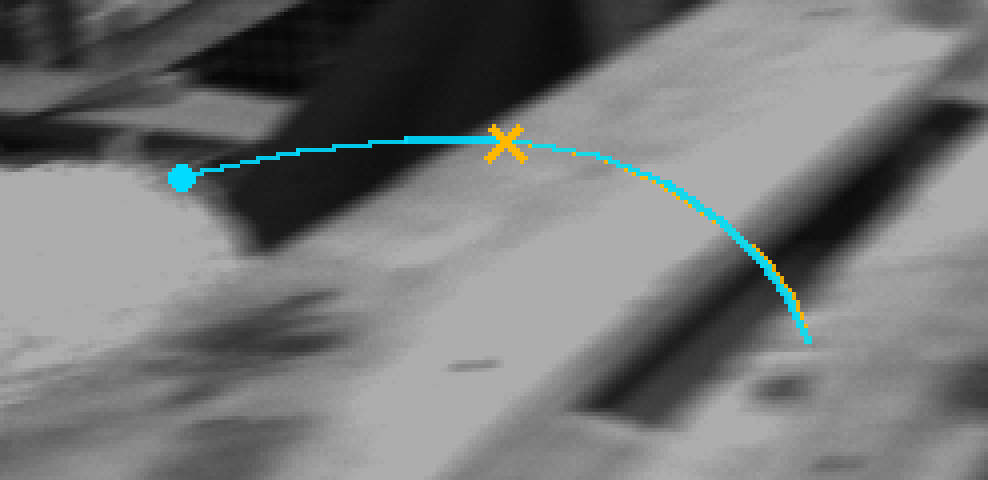
\includegraphics[width=\linewidth]{figures/method/mv-stop-combined}
  \end{minipage}\hfill
  \begin{minipage}[t]{0.485\textwidth}\centering
    \textbf{First unsupported transition}\\[-0.15em]
    {\small nearest raw-MV support is $6.0$ px away}\par\smallskip
    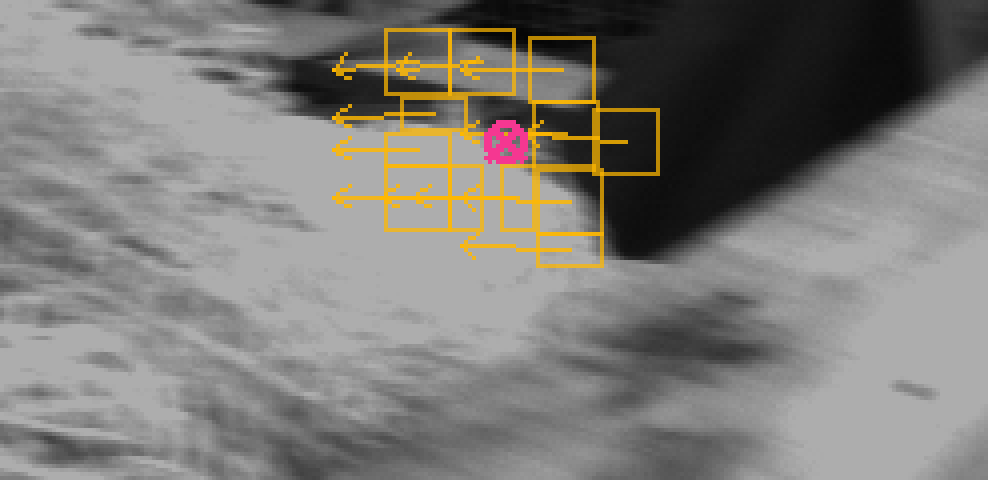
\includegraphics[width=\linewidth]{figures/method/mv-stop-neighborhood}
  \end{minipage}
  \caption[Abrupt local loss of codec support]{Abrupt local loss of codec support on EMH01. Orange and cyan have
  the same meanings as in \autoref{fig:mv-feature-departure-example}. The raw
  MV path follows the KLT diagnostic for six transitions and then terminates;
  the left panel places both complete paths on one image. The right panel shows
  a nearby subsample of the raw H.264 source supports and displacements used for
  the next transition. Other vectors are present locally, but none covers the
  propagated query marked in magenta. Decoded intensities are used only to
  construct this explanatory diagnostic.}
  \label{fig:mv-abrupt-stop-example}
\end{figure}

These two observations motivate reciprocal and geometric validation; neither
post-hoc KLT track is an additional pixel-domain gate in the method.

\section{Forward-Backward Consistency}

Tracking a point forward and then backward should return to its starting location when both estimates describe the same correspondence. Kalal et al. use this time-reversal principle to detect tracking failures from forward-backward error~\cite{kalal2010forwardbackward}. Zouein et al. apply a related directional-consistency test to tracks assembled from AV1 motion vectors~\cite{zouein2025leveraging}. Here the principle is adapted to H.264 block supports rather than image-tracked points.

Let $\mathbf{v}_f$ be a forward motion vector and let $\mathbf{v}_b$ be a vector from the reverse encoding, expressed in the same temporal direction. A candidate pair is retained only if its source and destination support rectangles overlap in both directions and
\begin{equation}
  \frac{\mathbf{v}_f^{\mathsf T}\mathbf{v}_b}
       {\lVert\mathbf{v}_f\rVert\lVert\mathbf{v}_b\rVert}
  \geq 0.98,
  \qquad
  \lVert\mathbf{v}_f-\mathbf{v}_b\rVert_2 \leq 1.5\ \text{px}.
\end{equation}
The minimum intersection-over-union of the corresponding source and destination supports must additionally be at least $0.15$. Two zero-displacement vectors are treated as directionally consistent. The validated support is the intersection that remains after translating both block supports into a common frame.

The retained hybrid policy uses reciprocal candidates for consensus estimation and continuation of established tracks. The larger best-direction pool may propose new tracks, but these remain provisional until a reciprocal continuation confirms a third observation. If only one encoding direction is available at an I-frame boundary, that direction is used as a fallback.

\begin{figure}[htbp]
  \centering
  \begin{minipage}[t]{0.315\textwidth}\centering
    \textbf{Forward: $64.78$ px}\par\smallskip
    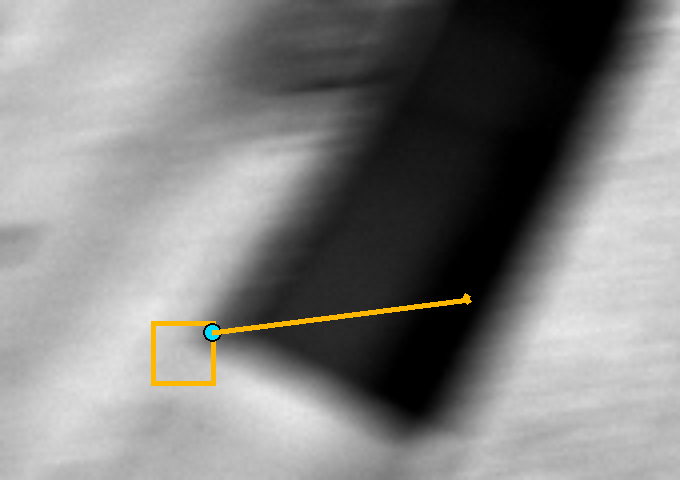
\includegraphics[width=\linewidth]{figures/method/reciprocal-accepted-1}
  \end{minipage}\hfill
  \begin{minipage}[t]{0.315\textwidth}\centering
    \textbf{Reverse: $65.03$ px}\par\smallskip
    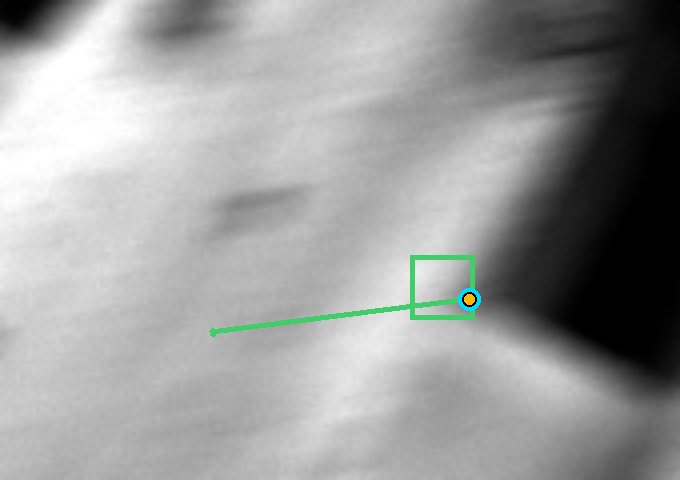
\includegraphics[width=\linewidth]{figures/method/reciprocal-accepted-2}
  \end{minipage}\hfill
  \begin{minipage}[t]{0.315\textwidth}\centering
    \textbf{Cycle closure: $0.25$ px}\par\smallskip
    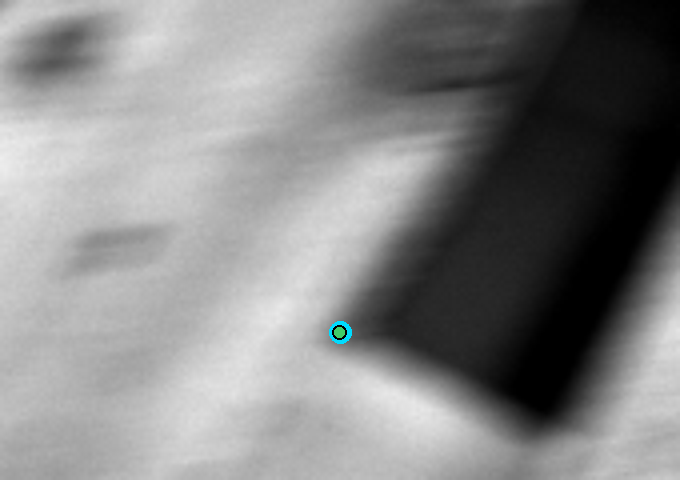
\includegraphics[width=\linewidth]{figures/method/reciprocal-accepted-3}
  \end{minipage}

  {\small cosine $1.000$, IoU $0.31$; codec/KLT endpoint difference $0.13$ px}
  \caption[Accepted reciprocal motion-vector correspondence]{An accepted large-displacement reciprocal match on EMH01. The cyan marker identifies a post-hoc KLT
  feature, the orange arrow is the forward codec motion, and the green arrow is
  the reverse-encoding motion. In the middle panel, the cyan KLT ring encloses
  the orange codec endpoint; in the final panel, the green return point lies
  within $0.25\,\mathrm{px}$ of the cyan source point. The KLT observation also
  passes its own forward-backward check with $0.06\,\mathrm{px}$ error. Image
  intensities are used only for this explanatory validation and are not inputs
  to reciprocal correspondence selection.}
  \label{fig:reciprocal-example}
\end{figure}

\section{Robust Association and Track Identity}

For a temporal candidate $(\mathbf{u}_{t-1},\mathbf{u}_t)$, compressed-domain
stereo supplies the distance $\lambda$ along the native anchor-camera bearing
at each endpoint. Let $\hat{\mathbf b}_A(\mathbf u)$ denote the corresponding
unit bearing. These ranges and bearings form a putative 3D-3D association
\begin{equation}
  \mathbf{a}_i = \lambda_{t-1,i}\,\hat{\mathbf b}_A(\mathbf{u}_{t-1,i}),
  \qquad
  \mathbf{b}_i = \lambda_{t,i}\,\hat{\mathbf b}_A(\mathbf{u}_{t,i}).
\end{equation}
Under the static-scene assumption, the inlier pairs share one rigid transformation. TEASER++ estimates this consensus with fixed scale and a $0.1\,\mathrm{m}$ noise bound~\cite{yang2020teaser}. Each candidate is then tested against the estimated transform. For points beyond $5\,\mathrm{m}$, a further $1.5\,\mathrm{px}$ reprojection gate rejects associations whose metric residual is small only because of weak depth geometry. If registration fails, no temporal association is accepted for that frame.

An accepted continuation inherits the existing landmark ID. A new association receives a provisional ID and is withheld from the backend until the following frame confirms it. TEASER++ therefore acts as an association filter; its frame-to-frame transform is not inserted as a camera-pose measurement.

\begin{figure}[htbp]
  \centering
  \begin{minipage}[t]{0.475\textwidth}\centering
    \textbf{Accepted: source}\\[-0.15em]
    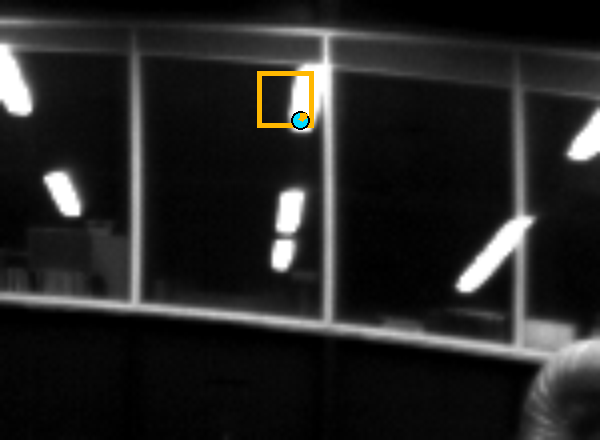
\includegraphics[width=\linewidth]{figures/method/teaser-accepted-source}
  \end{minipage}\hfill
  \begin{minipage}[t]{0.475\textwidth}\centering
    \textbf{Accepted: destination}\\[-0.15em]
    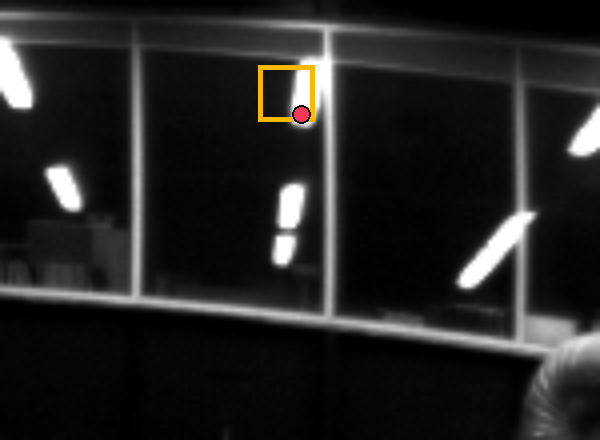
\includegraphics[width=\linewidth]{figures/method/teaser-accepted-destination}
  \end{minipage}\par\vspace{0.45em}
  \begin{minipage}[t]{0.475\textwidth}\centering
    \textbf{Rejected: source}\\[-0.15em]
    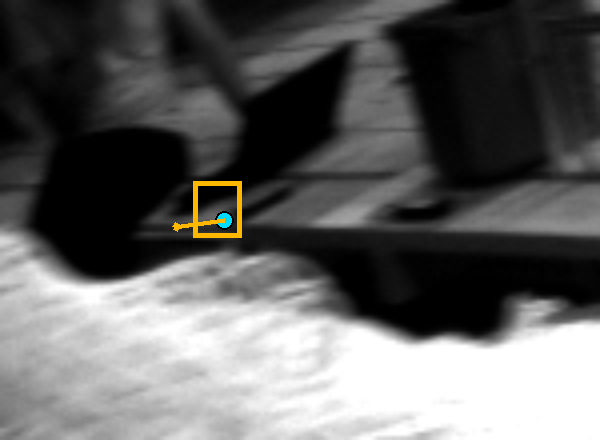
\includegraphics[width=\linewidth]{figures/method/teaser-rejected-source}
  \end{minipage}\hfill
  \begin{minipage}[t]{0.475\textwidth}\centering
    \textbf{Rejected: destination}\\[-0.15em]
    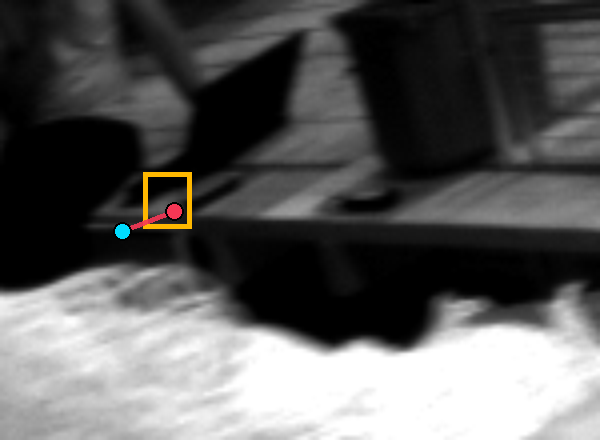
\includegraphics[width=\linewidth]{figures/method/teaser-rejected-destination}
  \end{minipage}
  \caption[Accepted and rejected robust-association candidates]{Individual robust-association decisions on EMH01. Orange outlines
  show the exact codec-block support, cyan marks a post-hoc KLT endpoint, and
  magenta marks the codec-motion endpoint. The accepted example has a
  $0.12\,\mathrm{px}$ endpoint difference. In the rejected example, the distinctly localized corner
  moves to the cyan position while the codec candidate ends
  $13.8\,\mathrm{px}$ away. Both KLT observations pass a one-pixel
  forward-backward check. KLT is used only to explain the decisions after
  estimation; TEASER++ receives the stereo 3D-3D candidates and no image data.}
  \label{fig:teaser-example}
\end{figure}

\section{Suppression of Indistinguishable Measurements}

Conventional feature frontends suppress nearby detections to avoid repeatedly representing the same local structure and to preserve spatially useful support~\cite{qin2018vins,kuhne2025lowlatency}. Codec blocks have no image-derived detector response on which to perform conventional non-maximum suppression. The proposed frontend instead suppresses measurements that cannot be distinguished at its available geometric resolution.

H.264 represents motion vectors at quarter-pixel precision and assigns each
vector to an extended prediction block. This finite spatial resolution motivates
treating sufficiently similar codec-derived observations as duplicate support.
Two accepted measurements are considered duplicates when their positions at both
temporal endpoints differ by at most $1.125\,\mathrm{px}$ in the $L_\infty$ norm
and their depth intervals overlap at both endpoints.

The interval model assigns a single-endpoint tolerance of $0.5625\,\mathrm{px}$,
half the selected suppression distance, giving a stereo-disparity tolerance of
$1.125\,\mathrm{px}$. It forms a disparity surrogate $f_xB/\lambda$ from the
triangulated camera range, perturbs it by the disparity tolerance, and maps the
limits back through the pinhole depth relation. A nonpositive lower disparity
limit gives an unbounded upper range limit. This is a pinhole approximation for
comparing depth support. The tolerances were selected in the parameter study;
quarter-pixel representation alone does not establish a bound on physical
correspondence error.

Candidates are processed in age order: established IDs are considered before new
births, and monotonically assigned IDs order older tracks first. The oldest
eligible representative is retained and suppresses younger indistinguishable
candidates. This favors continuity without inspecting image intensities.

\begin{figure}[htbp]
  \centering
  \begin{minipage}[t]{0.235\textwidth}\centering
    \textbf{Birth}\\[-0.15em]
    {\small $d_\infty=16.25$ px}\par\smallskip
    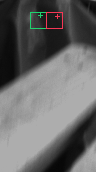
\includegraphics[width=\linewidth]{figures/method/suppression-retained-1}
  \end{minipage}\hfill
  \begin{minipage}[t]{0.235\textwidth}\centering
    \textbf{Age 4}\\[-0.15em]
    {\small $d_\infty=16.00$ px}\par\smallskip
    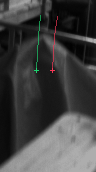
\includegraphics[width=\linewidth]{figures/method/suppression-retained-2}
  \end{minipage}\hfill
  \begin{minipage}[t]{0.235\textwidth}\centering
    \textbf{Age 7}\\[-0.15em]
    {\small $d_\infty=16.00$ px}\par\smallskip
    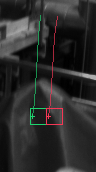
\includegraphics[width=\linewidth]{figures/method/suppression-retained-3}
  \end{minipage}\hfill
  \begin{minipage}[t]{0.235\textwidth}\centering
    \textbf{Age 10}\\[-0.15em]
    {\small $d_\infty=15.75$ px}\par\smallskip
    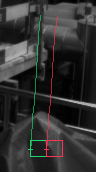
\includegraphics[width=\linewidth]{figures/method/suppression-retained-4}
  \end{minipage}
  \caption[Retention of nearby distinguishable tracks]{Two nearby but distinguishable EMH01 tracks over their complete
  ten-frame shared lifetime. Green and magenta identify the two retained IDs;
  the trails show their preceding image-plane observations. The centers are
  $16.25$ pixels apart at birth and remain between $15.75$ and $16.25$ pixels
  apart while moving approximately $135$ pixels through the image. Both IDs
  therefore survive age-prioritized suppression. This illustrates that the
  method does not enforce generic spatial sparsity: it removes only pairs that
  meet the $1.125$ pixel and depth-overlap criteria. Rectangles show the exact
  H.264 block dimensions rather than enlarged display regions.}
  \label{fig:suppression-example}
\end{figure}

\begin{figure}[htbp]
  \centering
  \begin{minipage}[t]{0.235\textwidth}\centering
    \textbf{Birth}\\[-0.15em]
    {\small $d_\infty=4.50$ px}\par\smallskip
    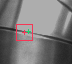
\includegraphics[width=\linewidth]{figures/method/suppression-merged-1}
  \end{minipage}\hfill
  \begin{minipage}[t]{0.235\textwidth}\centering
    \textbf{Age 2}\\[-0.15em]
    {\small $d_\infty=4.25$ px}\par\smallskip
    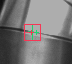
\includegraphics[width=\linewidth]{figures/method/suppression-merged-2}
  \end{minipage}\hfill
  \begin{minipage}[t]{0.235\textwidth}\centering
    \textbf{Age 3}\\[-0.15em]
    {\small $d_\infty=1.75$ px}\par\smallskip
    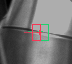
\includegraphics[width=\linewidth]{figures/method/suppression-merged-3}
  \end{minipage}\hfill
  \begin{minipage}[t]{0.235\textwidth}\centering
    \textbf{Age 4}\\[-0.15em]
    {\small younger ID suppressed}\par\smallskip
    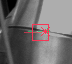
\includegraphics[width=\linewidth]{figures/method/suppression-merged-4}
  \end{minipage}
  \caption[Suppression of an indistinguishable younger track]{An age-prioritized suppression event recorded at the original
  $2.25$-pixel component-ablation setting on EMH01. The two
  accepted tracks are distinguishable at birth, approach one another, and end
  $1.75$ pixels apart for two consecutive observations. The older green ID is
  retained; the crossed magenta ID is omitted once the endpoint and
  depth-overlap tests both identify the measurements as indistinguishable. The
  selected PVO setting applies the same rule with a $1.125$-pixel bound.}
  \label{fig:suppression-merged-example}
\end{figure}

\section{Rigid-Flow Bundle Adjustment}

\subsection{Observation Model}

Conventional bundle adjustment treats an image coordinate
$\mathbf{u}_{j,t}^{c}$ as a noisy observation of a projected landmark,
\begin{equation}
  \mathbf{e}_{j,t}^{c}
  = \widehat{\mathbf{u}}_{j,t}^{c}-\mathbf{u}_{j,t}^{c},
  \qquad
  \widehat{\mathbf{u}}_{j,t}^{c}
  = \pi_c\!\left(\mathbf{T}_{WC_t}^{-1}\mathbf{p}_j^W\right).
\end{equation}
A codec block instead supplies a displacement over an extended prediction
region, without identifying a particular scene point within that region.
For an anchor-camera track propagated from an initial sample, the stored
coordinate after several accepted displacements is
\begin{equation}
  \mathbf{u}_{j,t}^{c}
  = \mathbf{u}_{j,0}^{c}+\sum_{k=1}^{t}\mathbf{m}_{j,k}^{c}.
\end{equation}
Absolute reprojection assigns each resulting coordinate a point-observation
residual. An earlier block-selection or displacement error can therefore affect
several later residuals. A fixed per-observation variance does not represent
this temporal correlation; it does not, however, imply that the coordinates
are assumed noise-free.

The evaluated alternative replaces eligible absolute factors with displacement
factors. Let $s$ be the predecessor timestamp explicitly recorded for
observation $(j,t,c)$. In the evaluated frontend this is the preceding processed
frame when the same ID has a stored observation in that camera. It is not
reassigned to an older retained keyframe if that predecessor is removed.
The shared landmark and two poses predict
\begin{equation}
  \Delta\widehat{\mathbf{u}}_{j,t}^{c}
  = \widehat{\mathbf{u}}_{j,t}^{c}
    -\widehat{\mathbf{u}}_{j,s}^{c},
\end{equation}
while the recorded measurement is
\begin{equation}
  \mathbf{m}_{j,t}^{c}
  = \mathbf{u}_{j,t}^{c}-\mathbf{u}_{j,s}^{c}.
\end{equation}
The rigid-flow residual is their difference,
\begin{equation}
  \mathbf{r}_{j,t}^{c}
  = \Delta\widehat{\mathbf{u}}_{j,t}^{c}-\mathbf{m}_{j,t}^{c}.
  \label{eq:rigid-flow-residual}
\end{equation}
Here \emph{rigid flow} means the image displacement predicted by reprojecting
one static landmark through two camera poses. It is not an additional measured
3D motion. The factor constrains a difference of projections without attaching
either endpoint to an absolute codec sample. Other factors still provide
absolute constraints, as detailed below. Shared poses and one persistent
landmark state couple the available temporal factors across a track.
This construction changes the observation model; it neither makes codec
correspondences exact nor removes the possibility of accumulated pose drift.

In the evaluated implementation, the frontend records the predecessor and
endpoint difference separately for each camera whenever both same-ID samples
are present. Anchor-camera samples are propagated using the selected temporal
motion vector. Stereo-camera samples are obtained from codec-stereo
correspondences and expressed in native stereo-camera pixels. Their stored
endpoint difference supplies $\mathbf{m}_{j,t}^{S}$; it is not a separately
queried temporal vector from the stereo camera. When both camera factors are
available, they share a landmark and pose pair but use their respective
calibrated projections. Missing flow metadata, including for some backfilled
birth observations, leaves an absolute observation instead.
\autoref{fig:absolute-versus-rigid-flow} illustrates the two observation models.

\begin{figure}[p]
  \centering
  \resizebox{!}{0.74\textheight}{%
  \begin{tikzpicture}[
      plane/.style={draw=TUMDarkGray,fill=TUMBlue!5,line width=0.45pt},
      sphere/.style={draw=TUMDarkGray!45,densely dotted},
      ray/.style={draw=TUMDarkGray!65,densely dotted},
      measured/.style={->,very thick,color=TUMAccentOrange},
      predicted/.style={->,very thick,color=TUMBlue},
      residual/.style={->,thick,color=red!75!black},
      artificial/.style={rectangle,draw=TUMAccentOrange,
        fill=TUMAccentOrange,inner sep=2.2pt}]
    \begin{scope}
      \node[font=\bfseries] at (2.5,5.05) {Absolute reprojection};
      \coordinate (P) at (2.5,2.70);
      \draw[sphere] (P) circle[radius=1.72];
      \fill[black] (P) circle[radius=2.3pt];
      \node[font=\small,above right] at (P) {$\mathbf p^W$};

      \begin{scope}[shift={(1.28,1.48)},rotate=-44]
        \path[plane] (-0.70,-0.22) -- (0.64,-0.15) --
          (0.70,0.22) -- (-0.64,0.15) -- cycle;
        \coordinate (p0) at (-0.12,0.00);
        \node[circle,fill=TUMBlue,inner sep=2.2pt] at (p0) {};
        \coordinate (a0) at (0.18,0.07);
        \node[artificial] at (a0) {};
      \end{scope}
      \begin{scope}[shift={(2.5,4.35)}]
        \path[plane] (-0.70,-0.20) -- (0.64,-0.13) --
          (0.70,0.20) -- (-0.64,0.13) -- cycle;
        \coordinate (p1) at (-0.16,0.00);
        \node[circle,fill=TUMBlue,inner sep=2.2pt] at (p1) {};
        \coordinate (a1) at (0.23,0.06);
        \node[artificial] at (a1) {};
      \end{scope}
      \begin{scope}[shift={(3.72,1.48)},rotate=44]
        \path[plane] (-0.70,-0.22) -- (0.64,-0.15) --
          (0.70,0.22) -- (-0.64,0.15) -- cycle;
        \coordinate (p2) at (-0.10,0.00);
        \node[circle,fill=TUMBlue,inner sep=2.2pt] at (p2) {};
        \coordinate (a2) at (0.28,0.07);
        \node[artificial] at (a2) {};
      \end{scope}
      \draw[ray] (P) -- (p0);
      \draw[ray] (P) -- (p1);
      \draw[ray] (P) -- (p2);
      \draw[measured] (a0) -- (a1);
      \draw[measured] (a1) -- (a2);
      \draw[residual] (a0) -- node[below,font=\scriptsize,inner sep=0.4444em] {$\mathbf e_{t-1}$} (p0);
      \draw[residual] (a1) -- node[above,font=\scriptsize,inner sep=0.4444em] {$\mathbf e_t$} (p1);
      \draw[residual] (a2) -- node[right,xshift=6pt,yshift=-2.3333pt,font=\scriptsize] {$\mathbf e_{t+1}$} (p2);
      \node[font=\scriptsize] at (0.62,0.72) {$\Pi_{t-1}$};
      \node[font=\scriptsize] at (1.62,4.35) {$\Pi_t$};
      \node[font=\scriptsize] at (4.38,0.72) {$\Pi_{t+1}$};
    \end{scope}

    \begin{scope}[yshift=-5.7cm]
      \node[font=\bfseries] at (2.5,5.05) {Rigid-flow reprojection};
      \coordinate (Q) at (2.5,2.70);
      \draw[sphere] (Q) circle[radius=1.72];
      \fill[black] (Q) circle[radius=2.3pt];
      \node[font=\small,above right] at (Q) {$\mathbf p^W$};

      \begin{scope}[shift={(1.28,1.48)},rotate=-44]
        \path[plane] (-0.70,-0.22) -- (0.64,-0.15) --
          (0.70,0.22) -- (-0.64,0.15) -- cycle;
        \coordinate (q0) at (-0.12,0.00);
        \node[circle,fill=TUMBlue,inner sep=2.4pt] at (q0) {};
      \end{scope}
      \begin{scope}[shift={(2.5,4.35)}]
        \path[plane] (-0.70,-0.20) -- (0.64,-0.13) --
          (0.70,0.20) -- (-0.64,0.13) -- cycle;
        \coordinate (q1) at (-0.16,0.00);
        \node[circle,fill=green!60!black,inner sep=2.4pt] at (q1) {};
        \coordinate (m1) at (0.12,-0.12);
      \end{scope}
      \begin{scope}[shift={(3.72,1.48)},rotate=44]
        \path[plane] (-0.70,-0.22) -- (0.64,-0.15) --
          (0.70,0.22) -- (-0.64,0.15) -- cycle;
        \coordinate (q2) at (-0.10,0.00);
        \node[circle,fill=violet!85!black,inner sep=2.4pt] at (q2) {};
        \coordinate (m2) at (0.18,-0.13);
      \end{scope}
      \draw[ray] (Q) -- (q0);
      \draw[ray] (Q) -- (q1);
      \draw[ray] (Q) -- (q2);
      \draw[predicted] (q0) -- (q1);
      \draw[predicted] (q1) -- (q2);
      \draw[measured] (q0) -- (m1);
      \draw[measured] (q1) -- (m2);
      \draw[residual] (m1) -- node[right,font=\scriptsize,inner sep=0.4444em] {$\mathbf r_t$} (q1);
      \draw[residual] (m2) -- node[right,xshift=6pt,yshift=-2.3333pt,font=\scriptsize] {$\mathbf r_{t+1}$} (q2);
      \node[font=\scriptsize] at (0.62,0.72) {$\Pi_{t-1}$};
      \node[font=\scriptsize] at (1.62,4.35) {$\Pi_t$};
      \node[font=\scriptsize] at (4.38,0.72) {$\Pi_{t+1}$};
    \end{scope}
  \end{tikzpicture}}
  \caption[Absolute reprojection and rigid-flow residuals]{Schematic comparison for one static landmark observed at
  three consecutive times. Top: absolute factors compare propagated codec samples
  (orange squares) with individual projections. Bottom: rigid-flow factors compare
  predicted displacement (blue) with recorded displacement (orange).
  Red arrows follow the predicted-minus-measured residual convention.
  Connections between the drawn image planes indicate temporal coupling;
  displacement subtraction is performed in image-pixel coordinates, not in
  the page-space geometry of this illustration.}
  \label{fig:absolute-versus-rigid-flow}
\end{figure}

\subsection{Shared State and Jacobian Assembly}

The implementation stores each landmark in its host camera, using two bearing
parameters and inverse distance,
$\boldsymbol{\ell}_j=(\alpha_j,\beta_j,\rho_j)^{\mathsf T}$.
The unit bearing $\mathbf b(\alpha_j,\beta_j)$ and $\rho_j$ form the homogeneous
point
\begin{equation}
  \overline{\mathbf p}_{h,j}(\boldsymbol{\ell}_j)
    = \begin{bmatrix}\mathbf b(\alpha_j,\beta_j)\\ \rho_j\end{bmatrix},
  \qquad
  \widehat{\mathbf u}_{j,k}^{c}
    = \pi_c\!\left(\mathbf T_{kh}
             \overline{\mathbf p}_{h,j}(\boldsymbol{\ell}_j)\right).
\end{equation}
Here $\mathbf T_{kh}$ maps the landmark host camera to camera $c$ at time $k$;
it combines the host and target body poses with the fixed camera extrinsics.
Both projections use the same $\boldsymbol{\ell}_j$, rather than independently
parameterized points at $s$ and $t$.

The two predictions are functions of one joint optimization state containing
the host pose, predecessor pose, current pose, and shared landmark. Therefore
\begin{equation}
  \frac{\partial\mathbf r}{\partial\mathbf x}
    = \frac{\partial\widehat{\mathbf u}_{j,t}^{c}}{\partial\mathbf x}
      -\frac{\partial\widehat{\mathbf u}_{j,s}^{c}}{\partial\mathbf x}.
\end{equation}
This subtraction requires identical state columns, with zeros for variables
absent from a projection. It does not identify the predecessor and current
poses as one variable.

Basalt first differentiates a projection with respect to its local
host-to-target pose perturbation and the landmark
parameters~\cite{usenko2020visual}. Denote these derivatives by
$\mathbf D_k\in\mathbb R^{2\times6}$ and
$\mathbf L_k\in\mathbb R^{2\times3}$.
Let $\mathbf A_{kh}$ and $\mathbf A_{kk}$ map the absolute host and target
body-pose perturbations into that local relative-pose perturbation. For
distinct host, predecessor, and current poses, the residual blocks are
\begin{equation}
  \begin{aligned}
    \mathbf J_h &= \mathbf D_t\mathbf A_{th}
                  -\mathbf D_s\mathbf A_{sh},&
    \mathbf J_s &= -\mathbf D_s\mathbf A_{ss},\\
    \mathbf J_t &= \mathbf D_t\mathbf A_{tt},&
    \mathbf J_{\ell} &= \mathbf L_t-\mathbf L_s.
  \end{aligned}
  \label{eq:rigid-flow-block-jacobians}
\end{equation}
Current and predecessor pose terms are placed in separate columns.
Subtraction within one block occurs for the shared landmark and, after the
chain rule, the shared host pose. If a host and target use the same body pose,
their contributions accumulate in the same block. When both timestamp and
camera are identical, the relative transform is identity and its pose
derivatives are zero.

The backend retains Basalt's pose-linearization convention: the
$\mathbf A$ maps are evaluated at stored pose linearization points, while the
projection transform is updated from the current estimates when those points
are held fixed. The local projection derivatives are evaluated using that
transform and the current landmark. Thus the block assembly above also applies
when marginalization has fixed the pose reference points; it does not imply
that every derivative is recomputed at the latest pose estimate.

\subsection{Factor Allocation and Weighting}

Both cameras are enabled for rigid-flow factors in the evaluated configuration.
A current observation receives a flow factor only if it is not the landmark's
host-camera observation, its finite flow measurement identifies an earlier
observation of the same ID in the same camera, and both poses are in the active
state ordering. Otherwise, an active observation receives an absolute factor.
The allocation is exclusive: one observation is never represented by both
factors in the same joint problem. If a selected flow factor has an invalid
projection at either endpoint, it contributes no residual at that
linearization; this projection failure does not trigger an absolute fallback.
The nonlinear objective and the linear system implement the same residual
definition and structural selection rule in separate routines.

For joint-window visual factors, the Huber weight is computed from the
two-dimensional residual norm in pixels before scaling by the observation
standard deviation. Holding this weight fixed for each linearization gives
the weighted residual and Jacobian rows used in the linear system:
\begin{equation}
  w_H =
  \begin{cases}
    1, & \|\mathbf r\|\leq\delta,\\
    \delta/\|\mathbf r\|, & \|\mathbf r\|>\delta,
  \end{cases}
  \qquad
  \widetilde{\mathbf r}=\frac{\sqrt{w_H}}{\sigma}\mathbf r,
  \qquad
  \widetilde{\mathbf J}=\frac{\sqrt{w_H}}{\sigma}\mathbf J .
\end{equation}
The selected settings are $\sigma=4$ pixels and $\delta=0.5$ pixels. Absolute
and displacement factors use this same scalar weighting; the model does not
introduce a separate flow covariance or temporal error-correlation matrix.
The residual ablation changes only this backend factor allocation in joint
optimization and marginalization,
holding the frontend and other backend settings fixed.

\subsection{Optimization and Marginalization}

After the incoming pose and its observations have been inserted, a pose-only
initialization step uses absolute reprojection of already connected landmarks.
It performs two Gauss--Newton updates with small damping; its normal equations
use unweighted valid projection residuals. The robust weighting described above
applies to the subsequent joint optimization and marginalization, not to these
initialization updates. All of these coordinates come from codec metadata and
calibrated geometry, without consulting image intensities.

A keyframe is requested when the fraction of currently observed anchor-camera
IDs connected to landmarks falls below $0.8$, provided more than one frame has elapsed since
the previous keyframe. New landmarks are triangulated from multi-camera or
multi-frame observations. Joint optimization uses absolute square-root QR
linearization to eliminate landmark increments, then solves the damped reduced
pose system. This is one coupled window problem, not an independent pose fit
for each flow measurement.

After optimization, old non-keyframe poses and their observations are removed
before the marginalization system is constructed. The most recent pose is
retained, so a preceding non-keyframe can still participate in the next joint
solve before its removal. After marginalization, the retained state contains
at most seven keyframes plus the current pose if it is not already a keyframe;
the joint solve can temporarily contain additional poses. The configured
three-state limit belongs to the inertial estimator and is inactive here.

Square-root marginalization forms a prior from the existing prior and selected
landmarks hosted by departing keyframes or classified as lost. Those
landmarks use the same factor-allocation rule on the observations and poses
that remain at this stage. Surviving eligible flow factors can therefore enter
the prior, but the procedure does not preserve every historical flow factor:
removal of a predecessor can make an observation use absolute reprojection,
and there is no replacement flow edge to another retained frame. The
separately explored pre-marginalization outlier-removal step and second
optimization pass are disabled in the evaluated method.

\section{Integration and Frame Processing}

The retained hybrid policy separates continuation from birth. Established IDs
may continue only through reciprocal forward-backward candidates. The larger
union of forward and inverted-reverse candidates may propose births, allowing
coverage where one direction is preferable, but a new ID remains provisional
until a reciprocal observation confirms it in the following frame. The frontend
therefore buffers two frames before publishing them to the backend. Once
confirmed, the withheld observations for the first two frames and the third
observation are emitted with one ID. A provisional track that fails confirmation
is discarded. At shutdown, buffered frames are flushed in timestamp order, but
unconfirmed births are not promoted.

The per-frame procedure is summarized below.

\begin{center}
\begin{minipage}{0.97\textwidth}
\hrule
\vspace{0.35em}
\textbf{Algorithm 1:} Pixel-free processing of frame $t$.
\vspace{0.35em}
\hrule
\vspace{0.25em}
\begin{tabular}{@{}r@{\hspace{0.8em}}p{0.91\linewidth}@{}}
  1 & \textbf{Input:} temporal and stereo MVs, calibration, masks, tracks, and backend state. \\
  2 & \textbf{Output:} confirmed observations with IDs and updated state. \\
  3 & Normalize MVs; apply source, mask, bounds, and median checks. \\
  4 & Form best-direction birth and reciprocal continuation pools. \\
  5 & Obtain stereo at both endpoints; fit fixed-scale TEASER++ to spatially subsampled 3D pairs. \\
  6 & Retain candidates passing stereo, rigid-consensus, and far-depth gates. \\
  7 & \textbf{for} active IDs $j$, oldest first, \textbf{do} \\
  8 & \quad Select the reciprocal successor with minimum 3D residual. \\
  9 & \quad Continue $j$ and record both camera displacements if suppression retains it. \\
 10 & \textbf{end} \\
 11 & Allocate provisional IDs from unused birth candidates surviving suppression. \\
 12 & Confirm provisional IDs after a reciprocal third observation. \\
 13 & Release confirmed observations after the two-frame delay. \\
 14 & For released frames, optimize the current pose and update keyframes and landmarks. \\
 15 & Optimize the active window and marginalize as required. \\
\end{tabular}
\vspace{0.25em}
\hrule
\end{minipage}
\end{center}
